%The computational model of Lazy Shadowing has been continuously optimized to improve its scalability and efficiency, to eliminate vulnerability, and to reduce implementation complexity and overhead. This section presents the system design of Rejuvenating Shadows. 

%\subsection{Fault model}

Rejuvenating Shadows assumes a fail-stop fault model, whereby a failed process halts and its internal state and memory content are irretrievably 
lost~\cite{Schlichting1983}. Furthermore, we assume that the processor on which the failure occurred can be rebooted and used to start a new process\footnote{Equivalently, a spare processor can be used for this purpose.}. This assumption also holds for checkpointing/restart to ensure fair comparative analysis. 
 
%As demonstrated in~\cite{cui_2016_scalcom}, Lazy Shadowing is able to tolerate both hardware and software failures under the fail-stop fault model. In this work, we continue with the assumption of fail-stop model. In order to further improve resilience and efficiency, however, Rejuvenating Shadows differentiates between temporary failures and permanent failures. Temporary failures include memory bit flips, kernel panic, etc., and can be recovered by rebooting the machine, while permanent failures, such as failure in power supply and network switch, needs the device to be replaced in order to recover. Rejuvenating Shadows maximizes the resource utilization for resilience by adopting different strategies for different types of failures. 

%\subsection{Shadowing}
%\label{sec:shadow}
Rejuvenating Shadows is a shadow replication based fault tolerance model, which associates a shadow to each main process. To achieve fault tolerance, shadows execute simultaneously with the mains, but on different nodes. Furthermore, to save power, shadows execute at a lower rate than their associated mains.  When a main fails, the shadow increases its execution rate to speed up recovery. However, contrary to Lazy Shadowing, where a shadow substitutes for its failed main, Rejuvenating Shadows uses a shadow as a \textit{rescuer} to restore the state of the main to where it was before failure. Upon state restoration, both the main and its associated shadow are active, thereby bringing back the system to its original level of fault tolerance.

%The basic tenet of Shadowing is to associate with each main process a shadow process as a replica, and simultaneously execute them on different nodes to achieve fault tolerance. Normally the shadows run at a lower rate to save power and computing resources. When a main process fails, its associated shadow is promoted to assume the role of the failed main. 

%In this way, shadow processes are substitutes for mains in the case of failure. 
%In this work, however, we no longer limit the shadow to be a ``pure" replica of the main. When a failure occurs, we use the shadow as a rescuer instead of a substitute,  to restore the main to its state before failure, thereby bringing back the system to its original resilience.
%In this work, we deviate from the original concept of shadow as a replica~\cite{cui_2016_scalcom} and use the state of the shadow to restore the main to its state prior to the failure. 

%\subsection{Consistency}
%\label{sec:consistency}



%The SYNC message in Figure~\ref{fig:cons_protocol} is only used when there is potential non-determinism. This will be discussed in details in the next Section.
%We assume that only MPI operations can introduce non-determinism. MPI\_ANY\_SOURCE may result in different message receiving orders between a main and its shadow. To deal with this, we serialize MPI\_ANY\_SOURCE message receiving by having the main first do the receiving and then use a SYNC message to forward the message source information to its shadow, which then issues a receiving with the specific source. Other operations, such as MPI\_Wtime() and MPI\_Probe(), can be dealt with in a similar manner by forwarding the result from a main to its shadow.

%Multiple approaches can be used to reduce the execution rate of a shadow, including Dynamic Voltage and Frequency Scaling (DVFS), shadow collocation, or a combination thereof. 
%The use of DVFS, however, entails undesirable consequences, such as reduced reliability and limited control granularity. 
To reduce a shadow's execution rate, Dynamic Voltage and Frequency Scaling (DVFS) can be applied. 
Its effectiveness, however, may be markedly limited by the granularity of voltage control, the number of frequencies available, and the negative effects on reliability~\cite{Eyerman:2011:FDU:1952998.1952999}.  
An alternative approach to DVFS is to collocate multiple shadows on a single processor~\cite{cui_2016_scalcom}. The desired execution rate can be achieved by controlling the collocation ratio, defined as the number of shadows that time-share a processor. An example of 3 \textit{shadowed sets}, with a collocation ratio of 4, is depicted in Figure~\ref{fig:logical_org}. A shadowed set refers to a set of mains and their collocated shadows. 

\begin{figure}[!t]
  \begin{center}
      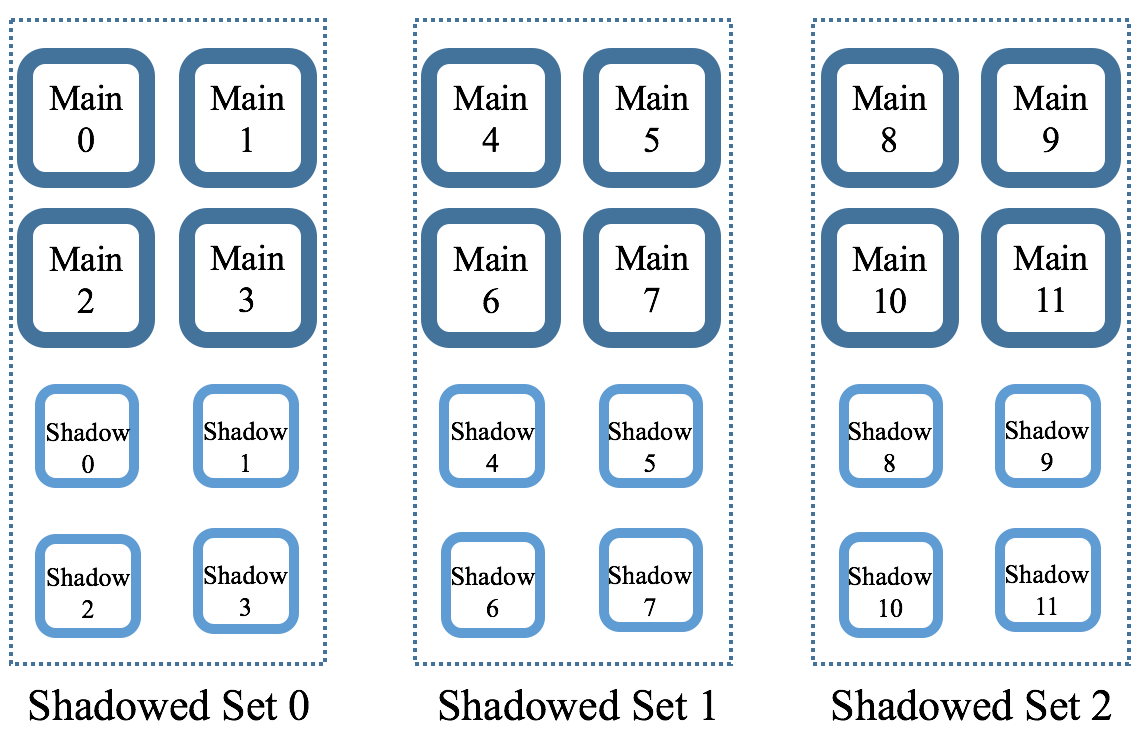
\includegraphics[width=\columnwidth]{figures/logical_org_hpcc}
  \end{center}
  \vskip -0.2in
  \caption{Logical organization of 12 mains and their shadows with every 4 shadows collocated, resulting in 3 shadowed sets.}
  \label{fig:logical_org}
  \vskip -0.25in
\end{figure}

Contrary to pure replication, shadow collocation reduces the number of processors required to achieve fault-tolerance, thereby reducing power and energy consumption. Furthermore, the collocation ratio can be adapted to reflect the propensity of the system to failure. This flexibility, however, comes at the increased cost of memory requirement at the shared processor. It is to be noted that this limitation is not intrinsic to Rejuvenating Shadows, as in-memory and multi-level checkpointing also require additional memory to store checkpoints. In this work, we only focus on collocation to reduce execution rate. 

%The term shadowed set refers to a set of mains whose associated shadows are collocated at the same processor.

In the basic form of shadow replication, failures can have a significant impact on the performance. Since a shadow executes at a lower rate than its associated main, a {\it divergence} is likely to occur between the pair of processes, as computation progresses. The impact of computational divergence on  time-to-completion can be prohibitive, as the time required for a lagging shadow to ``catch up"  with its associated main can be significant. Failures can also impact the resilience of the system. Upon failure of a main, the system can only rely on  an ``orphan" shadow to complete the task. A trivial approach to address this shortcoming is to associate a ``suite" of shadows with each main. Such an approach, however, is resource wasteful and costly in terms of energy consumption. To address the impact of computational divergence on system performance, while maintaining a persistent resilience level against multiple failures, two techniques, \textit{leaping} and \textit{rejuvenation}, are proposed.

\subsection{Leaping}

%Leaping was initially proposed as a technique to boost the performance of lazy shadows~\cite{cui_2016_scalcom}. 
The main objective of \textit{leaping} is to ensure forward progress in the presence of failure. As stated above, the failure of a main may cause the remaining processes to halt at a synchronization point, until the shadow associated with the failed main catches up. This process can increase significantly the time-to-completion of the task. Leaping takes  advantage of the idle time to synchronize the state of the shadows with that of their non-failed mains. 
%To mitigate this issue, we propose a technique, referred to as \textit{Leaping}, that takes advantage of the recovery time to synchronize the state of the shadows with that of their non-faulty mains. 
Leaping eliminates current divergence between non-failed mains and their associated shadows, with minimal computational and communication overhead. As such, it reduces significantly the recovery time of future failures. 
Leaping always takes place between a main and a shadow pair, and does not require global coordination. The process which provides the leaping state is referred to as the 
\textit{leap-provider},  while the rolling-forward process which receives the leaping state is referred to as the \textit{leap-recipient}. 


%With rejuvenation, we furter extend the concept of leaping to restore a failed process using the state of its associated process. In both cases, leaping takes between a pair of main and shadow. To avoid ambiguity, the process which provides state in a leaping is referred to as the target process, and the other process which receives and updates state is referred to as the roll forward process. 

%Recently, we have identified an empirical problem to which leaping is a solution. When Lazy Shadowing is used to execute an MPI application, application messages are generated at the rate of the mains, but consumed by the shadows at a lower rate because the shadows are slower. As a result, messages accumulate on the shadow side and could possibly result in a buffer overflow. Leaping is naturally a solution to this problem as it can move the shadows forward and synchronize their execution states with those of the mains. After the synchronization, accumulated messages at the shadows become obsolete and thus can be safely discarded. To differentiate the two cases where leaping is used, leaping during failure recovery is referred to as failure induced leaping while leaping to avoid buffer overflow is referred to as forced leaping. 

\subsection{Rejuvenation}

The main objective of rejuvenation is to enable the system to maintain its intended level of resilience, in the event of multiple failures\footnote{The case where both the main and shadow of a task fail simultaneously is not discussed specifically, as the occurrence of such an event is highly unlikely. Such failures can be handled by the shadow replication model by associating a suite of shadows to each main process.}. Based on the shadow replication model, when a main fails, its associated shadow increases its execution rate to catch up with the failed main. The execution rate increase is achieved by terminating  the remaining collocated shadows in the shadowed set, and allocating the processor to be used exclusively by the recovering shadow. Although efficient in reducing failure recovery time, this method reduces the execution of each task in the shadowed set to a single instance, thereby increasing the vulnerability of the system to subsequent failures. 
The proposed approach to address this shortcoming is to \textit{rejuvenate} the failed process, by launching a new process. Furthermore, rather than staring the newly launched process from its initial state, leaping is invoked to  synchronize the new process' state with that of its associated living process. A direct implication of rejuvenation is that collocated shadows no longer need to be terminated, but only suspended  until the recovery process is complete.  In addition to restoring  the system to its intended resilience level, rejuvenation also reduces the overall execution time. 


%When a main fails, its shadow increases its rate to speed up recovery. %In the case where the collocation ratio is greater than one, 
%With collocation, this is accomplished by terminating the other collocated shadows. As a result, however, only one instance of each task in the shadowed set remains, %. A subsequent fault in any task of this shadowed set will cause a system failure, 
%thereby making the shadow set vulnerable to future faults.This vulnerability can be avoided by using rejuvenation, whereby a new process is spawned for either a failed main or shadow, which eliminates the need for a shadow to permanently substitute for a main. As result, collocated shadows need not be terminated, but only temporarily suspended during the recovery process.  
%Upon recovery, every main is always guaranteed to have an associated shadow. The problem, however, is that the newly spawned process will start from its initial state and may lag far behind the other processes. When the new process needs to synchronize with other processes, significant delay will be incurred as a result of the lag. 

%The problem, however, is that the newly spawned process will start from its initial state and potentially delay the entire execution.
%Leaping provides the solution, with minimum overhead, 
%To deal with this issue, we extend the concept of leaping to synchronize the new process' state with that of its associated living shadow. 


%Consider a pair of main process, $M$, and shadow process, $S$, for example. If $M$ fails, a new main process will be started to replace $M$, and then a leaping from $S$ will advance the new process to the state of $S$. This is illustrated in Figure~\ref{fig:faulty}. 
Figure~\ref{fig:rejuvenation} illustrates the failure recovery process with rejuvenation, assuming that a main $M_i$ fails at time $T_0$.
In order for its shadow $S_i$ to speed up, the shadows collocated with $S_i$ are temporarily suspended. %, so that $S_i$ can increase its execution rate and finish the recovery as soon as possible. 
Meanwhile, the failed processor is rebooted and then a new process is launched for $M_i$. When, at $T_1$, $S_i$ catches up with the state of $M_i$ before its failure, leaping is performed to advance the new process to the current state of $S_i$. %The leaping is not initiated until $S_i$ catches up, since $M_i$ has already consumed the messages received before $T_0$ and, thus, should resume execution from where that execution was interrupted.
%so as to avoid the need of message logging. 

Because of the failure of $M_i$, the other mains are blocked at the next synchronization point, which is assumed to take place after $T_0$. During the idle time, a leaping is opportunistically performed to transfer state from each living main to its shadow. Therefore, this leaping has minimal overhead as it overlaps with the recovery, as shown in Figure~\ref{fig:non_faulty_diff}. Figure~\ref{fig:non_faulty_same} shows that leaping for the shadows collocated with $S_i$ are delayed until the recovery completes at $T_1$. After the leaping finishes at $T_2$, all mains and shadow resume normal execution with the same level of resilience as before the failure.

Figure~\ref{fig:rejuvenation} and the above analysis assume that the time for rebooting is no longer than the recovery time. If the new $M_i$ is not yet ready when $S_i$ catches up at $T_1$, however, two design choices are possible. In the first, $S_i$ can assume the role of a main and continue execution. In the second, $S_i$ can wait until the launching of the new $M_i$ is complete. The first option requires that all non-failed processes update their internal mapping to identify the shadow as a new main and continue to correctly receive messages (see Figure~\ref{fig:cons_protocol}). This not only complicates the implementation, but also requires expensive global coordination that is detrimental to scalability. We, therefore, chose the second design option.


%On the other hand, if $S$ fails, a new shadow process will be started and immediately advanced to the state of $M$ by leaping.

\begin{figure}[!t]
	\begin{center}
		\subfigure[Faulty task]
		{
			\label{fig:faulty}
			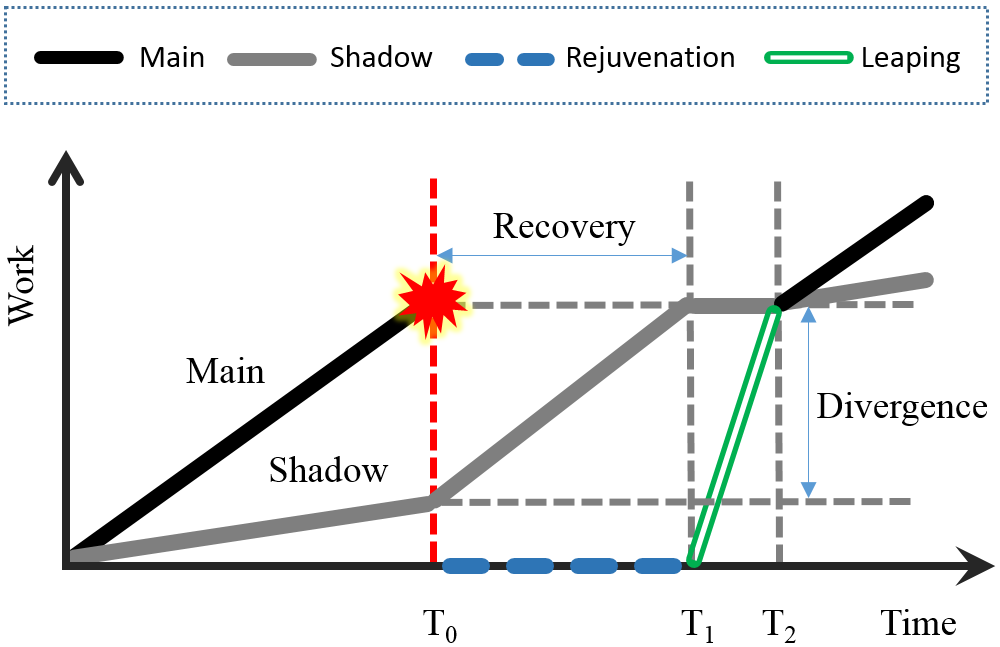
\includegraphics[width=0.7\columnwidth]{figures/rs1}
		}
		\subfigure[Non-faulty tasks in different shadowed sets]
		{
			\label{fig:non_faulty_diff}
			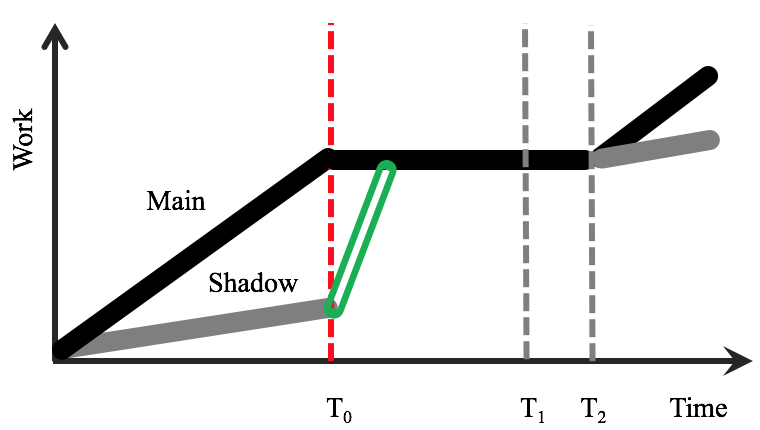
\includegraphics[width=0.7\columnwidth]{figures/rs2}
		}
		\subfigure[Non-faulty tasks in the same shadowed set]
		{
			\label{fig:non_faulty_same}
			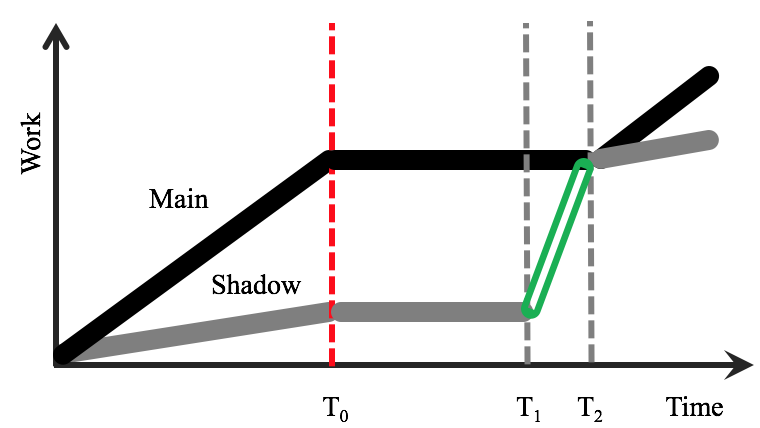
\includegraphics[width=0.7\columnwidth]{figures/rs3}
		}
	\end{center}
	\vskip -0.2in
	\caption{Recovery and rejuvenation after a main process fails.}
	\label{fig:rejuvenation}
\end{figure}

%Depending on the type of failure, the new process will be placed at different locations. If it is a temporary failure, the node where failure occurs will be rebooted and then used to host the new process, whether it is a main or shadow. Although there is a delay from the rebooting, it is usually small compared to application's running time and can be accounted part of the recovery. 
%For permanent failures, the node cannot be used and we have to migrate and collocate some processes. If the new process is a main, its existing shadow will be migrated to another node where shadow process(es) reside, and make room for the new main. Otherwise, if the new process is a shadow, it will be directly created on a shadow node. 
